\section{Opgave 2 - French flag}

\begin{enumerate}
\item[1)]

	
Vi vil i denne opgave skrive VHDL-koden til komponenten illustreret på figur \ref{fig:component}


Ved reverse-engineering, gennemgåes templaten som er udleveret, for at opnå en forståelse af dennes funktionalitet.
	
Først i arkitekturen sættes de faste grænser, som VGA-displayet må skrive i, som det ses i kodestykket \ref{lst:Template_Boundaries} nedenfor:
	\begin{lstlisting}[caption={Template Boundaries},label={lst:Template_Boundaries}]
-- horizontal Timing constants for 640 x 480 @ 60Hz
constant hFrontPorch : natural := 16; -- units are number of 25 MHz clocks
constant hBackPorch : natural := 48; 
constant hDataLen : natural := 640;
constant hSynWidth : natural := 96;

-- vertical Timing constants for 640 x 480 @ 60Hz 
constant vFrontPorch : natural := 10;  -- units are number of lines
constant vBackPorch : natural := 33;
constant vDataLen : natural := 480;
constant vSynWidth : natural := 2;

	\end{lstlisting}
	
Herpå oprettes signaler for de countere og flag som benyttes, for at holde styr på områderne der skal skrives i, af programmet, som det ses i kodestykket \ref{lst:Counters}:
\begin{lstlisting}[caption={Signal declaration},label={lst:Counters}]
-- signal declaration
signal hSyncCounter, vSyncCounter : integer range 0 to 1023; -- contrain integer to 10 bit.
signal hSyncOut,vSyncOut,clk25,vBlank,hBlank : std_logic;
\end{lstlisting}
	
Herpå halveres de 50 MHz til 25 MHZ allerførst i processen og vores egen procedure benyttes, trigget af forskellige clocks (hhv 25MHz signalet og hSyncOut).

Sidst findes koden for område-begrænsingen, der sætter farverne for diverse afgrænsede områder af flaget. Disse bliver bestemt ved farvekoderne inden for rød, grøn og blå.

\newpage
\item[2)]

Vi har fulgt underpunkterne i øvelses-vejledning og skrevet proceduren for \textit{\textbf{syncGenerator}} som det kan ses i figur \ref{lst:Procedure_code} fra linje 39:
\begin{lstlisting}[caption={syncGenerator Procedure Code},label={lst:Procedure_code}]

-- Template for VGA output by: Rene Kristensen
-- This design template uses gated clocks which generally are bad design practice.
-- This implies that the template design is not optimized for speed and will only serve for educational purpose. 
 
library ieee;
use ieee.std_logic_1164.all;
use ieee.numeric_std.all;

entity vga is
	port (clk,reset : in std_logic;
		  red, green, blue : out std_logic_vector(9 downto 0);
		  hsync, vsync, clockOut, blank, compSync: out std_logic);		
end vga;

architecture testGenerator of vga is

-- horizontal Timing constants for 640 x 480 @ 60Hz
constant hFrontPorch : natural := 16; -- units are number of 25 MHz clocks
constant hBackPorch : natural := 48; 
constant hDataLen : natural := 640;
constant hSynWidth : natural := 96;

-- vertical Timing constants for 640 x 480 @ 60Hz 
constant vFrontPorch : natural := 10;  -- units are number of lines
constant vBackPorch : natural := 33;
constant vDataLen : natural := 480;
constant vSynWidth : natural := 2;

-- signal declaration
signal hSyncCounter, vSyncCounter : integer range 0 to 1023; -- contrain integer to 10 bit.
signal hSyncOut,vSyncOut,clk25,vBlank,hBlank : std_logic;

-- attributes ensuring the signals defined below are not reduced away before simulation.
attribute keep: boolean; 						 -- don't reduce vSyncCounter and hSyncCounter signals away, so we can watch these signals i simulator
attribute keep of vSyncCounter : signal is true;  --   ||   --
attribute keep of hSyncCounter: signal is true;  --   ||   --

procedure syncGenerator(
signal syncCounter: inout integer range 0 to 1023 ; 
signal syncOut : out std_logic;
signal blankOut: out std_logic;
constant frontPorch : in natural;
constant backPorch : in natural;
constant dataLen : in natural;
constant syncWidth : in natural)
is
begin 
if 
syncCounter >= (frontPorch + backPorch + dataLen + syncWidth) then 
syncCounter<=0;
else 
syncCounter <= (syncCounter+1);
end if;
if 
(syncCounter > backPorch) and (syncCounter <= (backPorch+dataLen)) then
blankOut <= '0';
else 
blankOut <= '1';
end if;
if syncCounter>= (frontPorch+backPorch+dataLen) then
syncOut<='1';
else
syncOut <= '0';
end if;

end syncGenerator;

-- Your procedure should circular increment syncCounter, produce blanking and sync output.  

begin
clkdiv: process (reset,clk)  -- creates a 25 MHz pixel clock (clk25) from a 50 MHz input (clk).
begin
 if (reset = '0') then
   clk25 <= '0';
 elsif rising_edge(clk) then
   clk25 <= not clk25;
 end if; 
end process;

-- horizontal process using the generic syncGenerator function to generate a proper hsync pulse.
hsyn: process (reset,clk25) -- reacts on reset and 25 MHz clock.
begin
  if reset = '0' then
    hSyncCounter <= 0;
  elsif rising_edge(clk25) then
  syncGenerator(hSyncCounter,hSyncOut,hBlank,hFrontPorch,
  hBackPorch,hDataLen,hSynWidth); -- generates active low pulse after every line
  
  end if;
end process;

-- vertical process using the generic syncGenerator function to generate a proper vsync pulse.
vsyn: process (reset,hSyncOut) -- reacts on reset and hsync (meaning every line).
begin
  if reset = '0' then
    vSyncCounter <= 0;
  elsif rising_edge(hSyncOut) then
    syncGenerator(vSyncCounter,vSyncOut,vBlank,vFrontPorch,
    vBackPorch,vDataLen,vSynWidth); -- generates active low pulse after every picture
  end if;
end process;

color: process (reset, hSyncCounter,vSyncCounter)  -- draws italian flag color scheme
begin
  if ((hSyncCounter > hBackPorch) and (hSyncCounter <= hBackPorch+213)) then
    red   <= (others => '0');  -- Green
    green <= (others => '0');
    blue  <= (others => '1');  
  elsif ((hSyncCounter > hBackPorch+213) and (hSyncCounter <= hBackPorch+426)) then
    red   <= (others => '1');  -- White
    green <= (others => '1');
    blue  <= (others => '1');
  else
    red   <= (others => '1');  -- Red
    green <= (others => '0');
    blue  <= (others => '0');   
  end if;
end process;

vsync <= vSyncOut;				 -- connect vsync to entity
hsync <= hSyncOut;               -- connect hsync to entity
clockOut <= clk25;               -- 25 MHz clock for DAC 
blank <= not (vBlank or hBlank); -- active low blanking.
compSync <= '1'; 				 -- Never perform any composite sync. 
end testGenerator;

	\end{lstlisting}

\item[3)] 

Vi har downloadet programmet til DE2-boardet og opnår flaget som ses på figur \ref{fig:frenchFlag}.
	\begin{figure}[H]
		\centering
		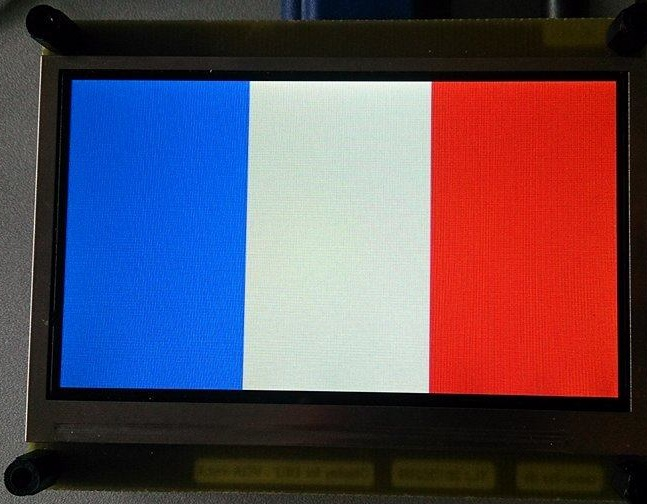
\includegraphics[scale=0.5]{pictures/Oevelse8/opg2/franskFlag}
		\caption{Det franske flag vist på VGA-skærmen}
		\label{fig:frenchFlag}
	\end{figure}
Ved at ændre på farvekoderne lavede vi også det Belgiske flag som vist på figur \ref{fig:belgiskflag}
\begin{figure}[H]
	\centering
	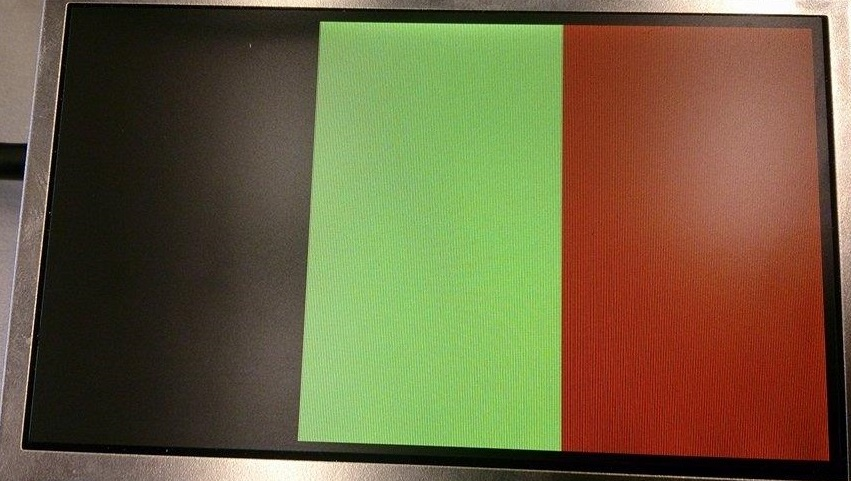
\includegraphics[scale=0.4]{pictures/Oevelse8/opg2/belgiskFlag}
	\caption{Det franske flag vist på VGA-skærmen}
	\label{fig:belgiskflag}
\end{figure}
\end{enumerate}